\documentclass[conference]{IEEEtran}
\IEEEoverridecommandlockouts
\usepackage{cite}
\usepackage{amsmath,amssymb}
\usepackage{graphicx}
\usepackage{booktabs}
\usepackage{url}
\usepackage{xcolor}

% Placeholders (PH of a key) are replaced by scripts/fill_tex.py from results/*.json.
\newcommand{\PH}[1]{\textcolor{red}{\texttt{#1}}}

\begin{document}

\title{An Equivalent-Key Chosen-Plaintext Break of a\\
2025 Chaos-Based Image Cipher}

\author{\IEEEauthorblockN{Author One, Author Two}
\IEEEauthorblockA{Department / Affiliation \\ City, Country \\ \{a1, a2\}@example.edu}}

\maketitle

\begin{abstract}
We cryptanalyse a recently published image-encryption scheme that combines Lorenz/logistic chaotic
maps with Fisher--Yates block shuffling (Jain \emph{et al.}, \emph{Optik}, 2025). We observe that the
scheme's keystream and both permutations depend only on the secret key and never on the image, so the
whole encryption is a fixed, plaintext-independent map. We reconstruct the cipher from its
description---matching its reported near-ideal entropy (e.g.\ \PH{cam_ent_cipher} on the Cameraman
image) and near-zero adjacent-pixel correlation---and then break it: an all-ones probe recovers the
per-position keystream and a few index-digit probes recover the permutation, so an equivalent key is
obtained in \PH{cam_cpt} chosen plaintexts and any ciphertext is decrypted pixel-exactly in
\PH{cam_attack_s}\,s without the key. We further show the scheme's headline differential metric is
illusory: because it applies no plaintext diffusion, a one-pixel change alters exactly one ciphertext
pixel, giving a true NPCR of \PH{cam_npcr1px}\,\% (i.e.\ $100/MN$), not the $\approx$99.6\,\% reported
(that figure merely reflects the difference between unrelated images, here \PH{npcr_unrelated}\,\%).
We conclude with the standard fixes.
\end{abstract}

\begin{IEEEkeywords}
cryptanalysis, image encryption, chaotic cipher, chosen-plaintext attack, equivalent key, NPCR
\end{IEEEkeywords}

\section{Introduction}
Chaos-based image ciphers are published in large numbers, and a recurring lesson from the
cryptanalysis literature is that many of them fall to the same structural attack: if the diffusion
keystream does not depend on the plaintext, the cipher reduces to a fixed permutation--substitution
map and an \emph{equivalent key} can be recovered from a handful of chosen
plaintexts~\cite{li2019attacker,li2018entropy,arroyo2009,li2011optimal}. Standard statistical scores
(entropy, correlation, NPCR/UACI) do not certify resistance to this attack, a point repeatedly made
but repeatedly ignored~\cite{alvarez2006}.

This paper applies that lesson to a 2025 scheme~\cite{jain2025lleo} (henceforth LLEO) built from the
Lorenz~\cite{lorenz1963} and logistic maps with Fisher--Yates block shuffling. Our contributions are:
(i) we identify that LLEO is entirely key-driven and therefore a fixed monomial map over
$\mathbb{Z}_{256}$; (ii) we give an equivalent-key chosen-plaintext attack that recovers the full map
in $1+\lceil\log_{256} MN\rceil$ chosen plaintexts and decrypts any image pixel-exactly without the
key; and (iii) we show that LLEO's near-ideal entropy and reported NPCR coexist with \emph{zero}
plaintext diffusion, so the claimed differential-attack resistance does not exist.

\section{The target cipher}
LLEO encrypts an $M\times N$ grayscale image in three key-driven steps. (1) \emph{Substitution.} The
image is split into 16 horizontal strips; odd strips are combined with a keystream $k_{\mathrm{log}}$
from the logistic map $x_{n+1}=rx_n(1-x_n)$ and even strips with a keystream $k_{\mathrm{lor}}$ from
the Lorenz system, via an invertible per-position operation (the paper inverts it with a modular
``conjugate''). (2) \emph{Permutation~1.} The 16 horizontal strips are reordered by a Fisher--Yates
shuffle. (3) \emph{Permutation~2.} The result is split into 16 vertical strips and shuffled again. The
four ``decryption keys'' are the two keystreams and the two shuffle index lists. Crucially, the
keystreams are seeded from key-dependent initial conditions and the shuffles from the key; \emph{no
quantity depends on the image}. The scheme is described as ``asymmetric,'' but the same data decrypts,
so it is a symmetric cipher.

\section{Cryptanalysis}
\subsection{Structural observation}
Writing the image as a length-$n$ vector ($n=MN$), every LLEO step is linear over $\mathbb{Z}_{256}$
and key-fixed: substitution multiplies coordinate $p$ by a unit $K[p]$, and the two block shuffles
compose into a single position permutation $P$. Hence
\begin{equation}
C[j] \;=\; K[s(j)]\,\cdot\,X[s(j)] \pmod{256},\qquad s=P^{-1},
\end{equation}
a fixed \emph{monomial} map: each ciphertext pixel is one plaintext pixel scaled by a fixed unit and
relocated. There is no constant term ($E(\mathbf{0})=\mathbf{0}$) and, decisively, no dependence on
$X$ beyond the single coordinate $s(j)$.

\subsection{Equivalent-key recovery}
Because $K$ and $s$ are fixed, two kinds of chosen plaintext suffice.
\emph{(a) Multiplier.} Encrypting the all-ones image gives $C[j]=K[s(j)]\cdot 1=K[s(j)]$, i.e.\ the
multiplier seen at every output position, in one query.
\emph{(b) Permutation.} Encrypting the plaintext whose pixel $i$ holds the $t$-th base-256 digit of
$i$ gives $C[j]=K[s(j)]\cdot \mathrm{digit}_t(s(j))$; dividing by the known multiplier yields
$\mathrm{digit}_t(s(j))$, so $\lceil\log_{256} n\rceil$ such queries reconstruct $s$.
The recovered $(s,K)$ form an equivalent key; any ciphertext is inverted by
$X[s(j)] = K[s(j)]^{-1} C[j]$. The cost is $1+\lceil\log_{256} n\rceil$ chosen plaintexts---%
\PH{cam_cpt} for a $512\times512$ image---independent of the key length the scheme advertises.

\section{Experimental results}
We reconstructed LLEO from its description and ran it on four standard $512\times512$ images.

\subsection{Reproduction}
Table~\ref{tab:repro} shows the reconstruction reproduces LLEO's claimed statistics: cipher entropy
approaches the ideal 8 (Cameraman \PH{cam_ent_cipher}, up from \PH{cam_ent_plain}) and adjacent-pixel
correlation drops to near zero (\PH{cam_corr_cipher}). Fig.~\ref{fig:hist} and
Fig.~\ref{fig:corr} show the flat cipher histogram and the destroyed correlation.

\begin{table}[t]
\centering
\caption{Reconstruction statistics and attack outcome (512$\times$512). Every image is recovered
pixel-exactly without the key.}
\label{tab:repro}
\begin{tabular}{lccccc}
\toprule
Image & $H$ plain & $H$ cipher & corr.\ cipher & chosen PT & broken \\
\midrule
Cameraman & \PH{cam_ent_plain} & \PH{cam_ent_cipher} & \PH{cam_corr_cipher} & \PH{cam_cpt} & yes \\
Moon      & \PH{moon_ent_plain} & \PH{moon_ent_cipher} & \PH{moon_corr_cipher} & \PH{moon_cpt} & yes \\
Gravel    & \PH{grv_ent_plain} & \PH{grv_ent_cipher} & \PH{grv_corr_cipher} & \PH{grv_cpt} & yes \\
Brick     & \PH{brk_ent_plain} & \PH{brk_ent_cipher} & \PH{brk_corr_cipher} & \PH{brk_cpt} & yes \\
\bottomrule
\end{tabular}
\end{table}

\subsection{The break}
The attack of Section~III recovers the equivalent key in \PH{cam_cpt} chosen plaintexts and decrypts a
fresh ciphertext pixel-exactly in \PH{cam_attack_s}\,s (Cameraman), using no key.
Fig.~\ref{fig:break} shows the original, the LLEO ciphertext, and the key-free recovery, which is
identical to the original.

\begin{figure}[t]
\centering
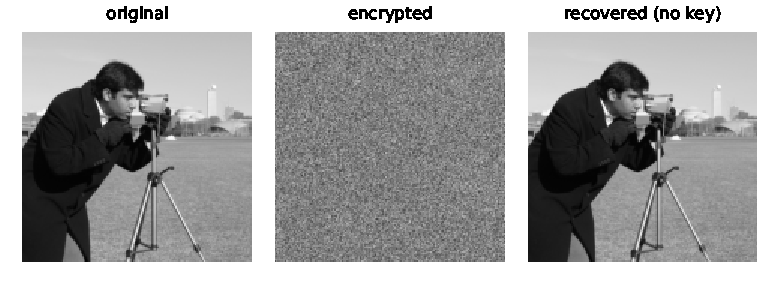
\includegraphics[width=0.98\columnwidth]{figures/break_cameraman.pdf}
\caption{Original, LLEO ciphertext, and the key-free recovery from \PH{cam_cpt} chosen plaintexts.}
\label{fig:break}
\end{figure}

\subsection{The differential metric is illusory}
LLEO reports NPCR $\approx$99.6\,\% as evidence of differential-attack resistance. But LLEO applies no
diffusion: each ciphertext pixel is a function of a single plaintext pixel, so flipping one plaintext
pixel changes exactly one ciphertext pixel. The true one-pixel NPCR is therefore $100/MN =
\PH{cam_npcr1px}\,\%$ (UACI \PH{cam_uaci1px}\,\%), not 99.6\,\%. The reported figure instead reflects
the difference between \emph{unrelated} images, which for LLEO is \PH{npcr_unrelated}\,\%---a quantity
every cipher achieves and which says nothing about chosen-plaintext security. Finally, the underlying
chaotic keystreams are themselves non-uniform: a chi-square test rejects uniformity for the logistic
keystream ($\chi^2=\PH{chi2_logistic}$, $p=\PH{p_logistic}$).

\begin{figure}[t]
\centering
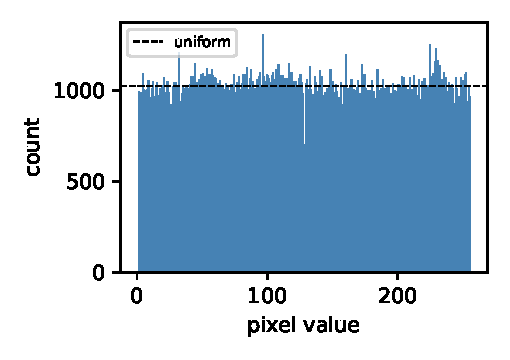
\includegraphics[width=0.7\columnwidth]{figures/cipher_hist.pdf}
\caption{Cipher histogram (Cameraman): near-uniform, yet the cipher is trivially broken.}
\label{fig:hist}
\end{figure}

\begin{figure}[t]
\centering
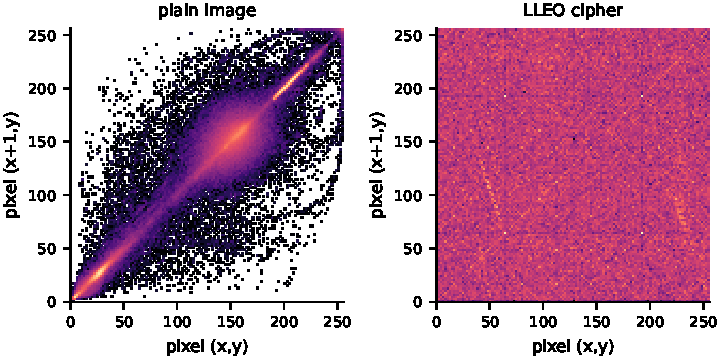
\includegraphics[width=0.92\columnwidth]{figures/correlation_scatter.pdf}
\caption{Adjacent-pixel correlation, plain vs.\ cipher (Cameraman).}
\label{fig:corr}
\end{figure}

\section{Discussion}
LLEO illustrates two persistent failure modes. First, \emph{good statistics are not security}: a flat
histogram, near-ideal entropy, and a large inter-image NPCR are all satisfied by our fixed
key-independent-of-plaintext map, which we nonetheless break in \PH{cam_cpt} queries. Second,
\emph{naming is not architecture}: calling a symmetric construction ``asymmetric'' does not add
security. The standard remedies are well known~\cite{alvarez2006,li2019attacker}: make the keystream
depend on the plaintext (e.g.\ seed the chaotic initial conditions from a cryptographic hash of the
image), and add genuine diffusion so that one plaintext change propagates across the ciphertext. With
a plaintext-dependent keystream the all-ones and digit probes no longer reveal a reusable equivalent
key, and the attack of Section~III fails.

\section{Conclusion}
A 2025 chaos-based image cipher is completely broken by an equivalent-key chosen-plaintext attack in
\PH{cam_cpt} chosen plaintexts and a fraction of a second, despite near-ideal entropy and a reported
NPCR of $\approx$99.6\,\%. The break follows directly from the cipher being key-only; its differential
metric, measured correctly, is \PH{cam_npcr1px}\,\%. We recommend plaintext-dependent keystreams and
real diffusion, and that statistical scores be reported alongside, not in place of, a chosen-plaintext
security argument.

\section*{Acknowledgment}
The authors used a large language model (Anthropic Claude) to assist with code, reproduction, and
editing. All claims were verified by the authors; the AI system is not an author. Generative-AI use is
disclosed per IEEE policy.

\bibliographystyle{IEEEtran}
\bibliography{references}

\end{document}
